\documentclass[aspectratio=169,mathserif]{beamer}
%\documentclass[aspectratio=169,mathserif,handout]{beamer}

\usepackage{graphicx} % Allows including images
\graphicspath{{./img/}}

\usepackage{epstopdf}
\epstopdfsetup{outdir=./img/}

\usepackage[utf8]{inputenc}
%Load useful packages
\usepackage{booktabs} % Allows the use of \toprule, \midrule and \bottomrule in tables
\usepackage{subcaption}
\usepackage{subfiles}
\usepackage{url}
\usepackage{amssymb}
%
\usepackage{multirow}
%
% align enum description
% \usepackage{enumitem}
% refs
\usepackage[style=authoryear,natbib=true]{biblatex}
\bibliography{references.bib}
%
\usepackage{tikz}
\usepackage{tikz-cd}
\usepackage{tikzscale}
\usetikzlibrary{calc,matrix,chains,positioning,decorations.pathreplacing,decorations.text,arrows,cd}

% overlays
\tikzset{
invisible/.style={opacity=0},
visible on/.style={alt={#1{}{invisible}}},
alt/.code args={<#1>#2#3}{%
\alt<#1>{\pgfkeysalso{#2}}{\pgfkeysalso{#3}} % \pgfkeysalso doesn't change the path
},
}

% neural nets
\tikzset{%
  every neuron/.style={
circle,
draw,
%minimum size=1cm
  },
  neuron missing/.style={
draw=none, 
scale=1,
text height=0.333cm,
execute at begin node=\color{black}$\vdots$
  },
}

% infrastructure
\tikzset{
vertex/.style = {
circle,
fill= black,
outer sep = 2pt,
inner sep = 1pt,
}
}




%Information to be included in the title page:
\title{Deep Learning}

\author{Tiago Vieira}
\institute{Institute of Computing\\Universidade Federal de Alagoas}
\date{\today}
%Logo in every slide
\logo{%
  \makebox[0.98\paperwidth]{

\includegraphics[width=0.5cm,keepaspectratio]{../logos/ufal_logo.png}%
\hfill%
\includegraphics[height=1cm,keepaspectratio]{logos/edge_logo.png}%

\includegraphics[height=0.8cm,keepaspectratio]{../logos/ic_logo.png}%
  }
}
%Contents before every section's starting slide
\AtBeginSubsection[]
{
  \begin{frame}
\frametitle{Summary}
\scriptsize
\tableofcontents[currentsection,currentsubsection]
  \end{frame}


}
% shape, colour of item, nested item bullets in itemize only
% \setbeamertemplate{itemize item}[square] \setbeamercolor{itemize item}{bg=blue}
% \setbeamertemplate{itemize subitem}[circle] \setbeamercolor{itemize subitem}{fg=green}
% \setbeamertemplate{itemize subsubitem}[triangle] \setbeamercolor{itemize subsubitem}{fg=red}
% font size of nested and nested-within-nested bulltes in both itemize and enumerate
% options are \tiny, \small, \scriptsize, \normalsize, \footnotesize, \large, \Large, \LARGE, \huge and \Huge
\setbeamerfont{itemize/enumerate subbody}{size=\scriptsize} 
\setbeamerfont{itemize/enumerate subsubbody}{size=\scriptsize}
% figure numbers
% \setbeamertemplate{caption}[numbered]
% blocks style
\setbeamertemplate{blocks}[rounded][shadow=true]


% Hide nav control
\usenavigationsymbolstemplate{}
% add numbering
\addtobeamertemplate{navigation symbols}{}{%
\usebeamerfont{footline}%
\usebeamercolor[fg]{footline}%
\hspace{1em}%
\insertframenumber/\inserttotalframenumber
}

% Footnote without number
\newcommand\blfootnote[1]{%
\begingroup
\renewcommand\thefootnote{}\footnote{#1}%
\addtocounter{footnote}{-1}%
\endgroup
}

% items symbols
\setbeamertemplate{itemize subitem}{-}
\setbeamertemplate{itemize subsubitem}{-}

%%setting up some useful slide creation commands
%split slide
% \newenvironment{splitframe}[5]
% %[1] ==> 1 parameter passed through {}
% %[2] ==> 2 parameters passed through {}{}
% %[4] ==> 4 parameters passed through {}{}{}{}
% {
% \begin{frame}{#3}
% \begin{columns}
% \column{#1\linewidth}
% \centering
% #4
% \column{#2\linewidth}
% \centering
% #5
% \end{columns}
% \centering
% \vspace{\baselineskip} % adds one line space
% }
% %Inside the first pair of braces (ABOVE) is set what your new environment will do before the text within, then inside the second pair of braces (BELOW) declare what your new environment will do after the text. Note second pair can be empty braces too.
% {
% \end{frame}


% }




\subtitle{Applications}

\begin{document}

\frame{\titlepage}

\begin{frame}{Outline}
\tableofcontents
\end{frame}

\section{Introduction}

\begin{frame}{Introduction}
\begin{figure}[!]
\centering
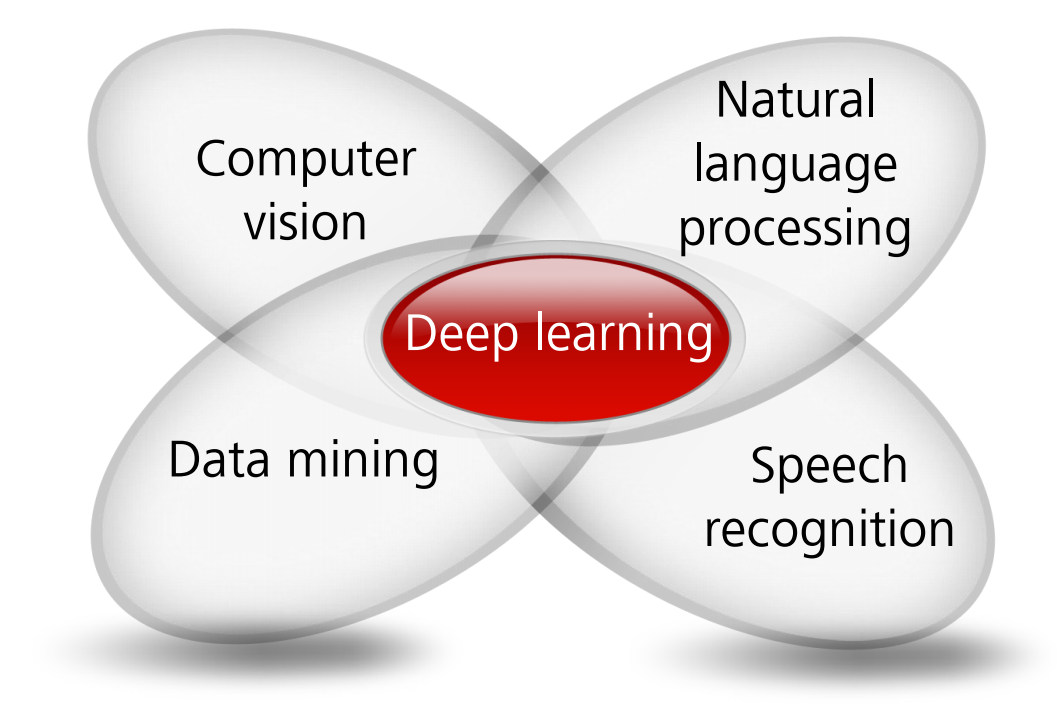
\includegraphics[width=.7\textwidth]{areas}
\end{figure}
\end{frame}

\section{Computer Vision}

\begin{frame}{Computer Vision}
\begin{columns}[t]
\begin{column}{.4\textwidth}
\begin{itemize}
\item Image classification.
\item Scene recognition.
\item Face detection and recognition.
\item Object detection and recognition.
\item Semantic segmentation.
\item Style transfer.
\item Super-resolution.
\item Optical Character Recognition (OCR).
\end{itemize}
\end{column}
\begin{column}{.6\textwidth}
\begin{figure}[!]
\centering
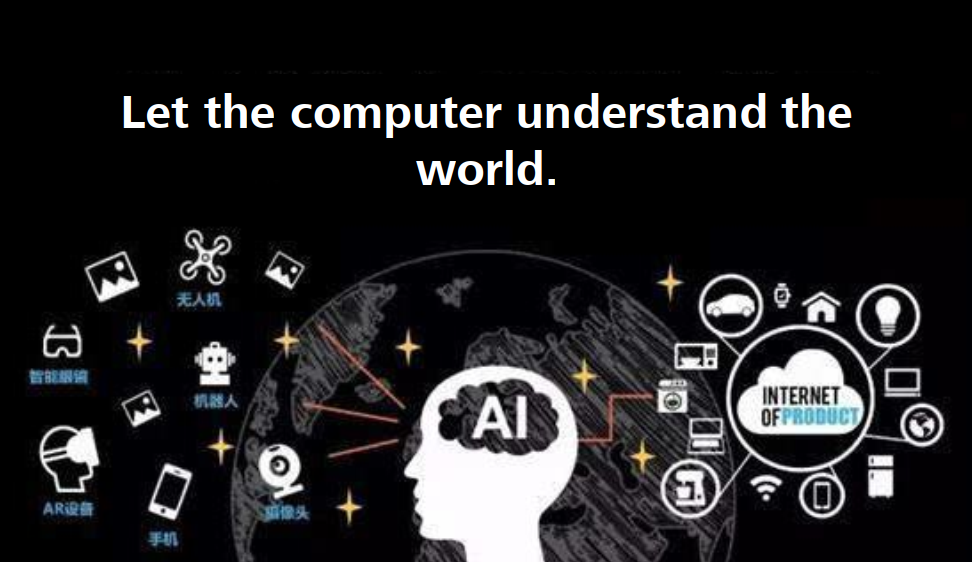
\includegraphics[width=\textwidth]{understand}
\end{figure}
\end{column}
\end{columns}
\end{frame}

%\subsection{Image Classification}

\begin{frame}{Image Classification}
Maps images to different class sets, which can be used for:
\begin{itemize}
\item image retrieval, and;
\item image archiving.
\end{itemize}
\begin{figure}[!]
\centering
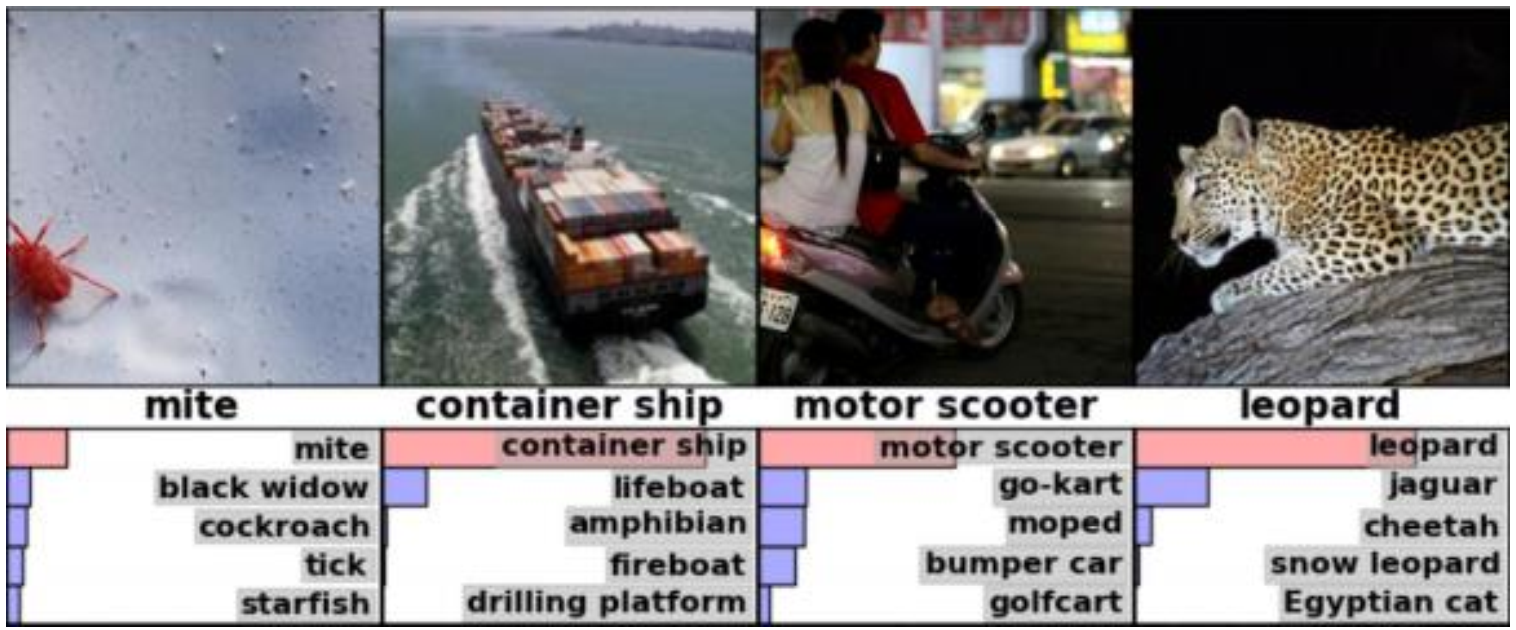
\includegraphics[width=\textwidth]{classification}
\end{figure}
\end{frame}

%\subsection{Scene Recognition}

\begin{frame}{Scene Recognition}
Classifies images based on scenes and environments, which can be used for situation awareness and intelligent 3A for photographing.
\begin{figure}[!]
\centering
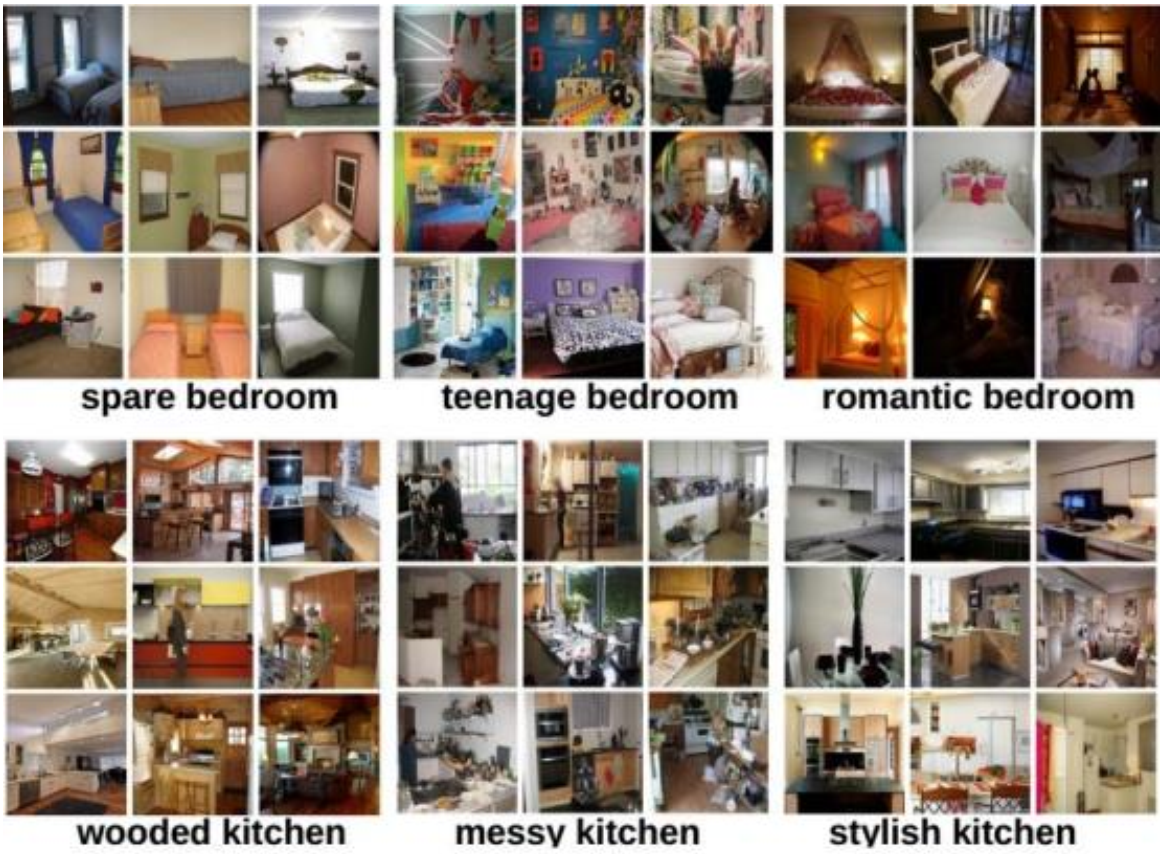
\includegraphics[width=.6\textwidth]{scene}
\end{figure}
\end{frame}

%\subsection{Face Detection and Recognition}

\begin{frame}{Face Detection}
Discovers and locates faces and facial features in images, which can be used for face focusing, polishing up, and augmented reality.
\begin{figure}[!]
\centering
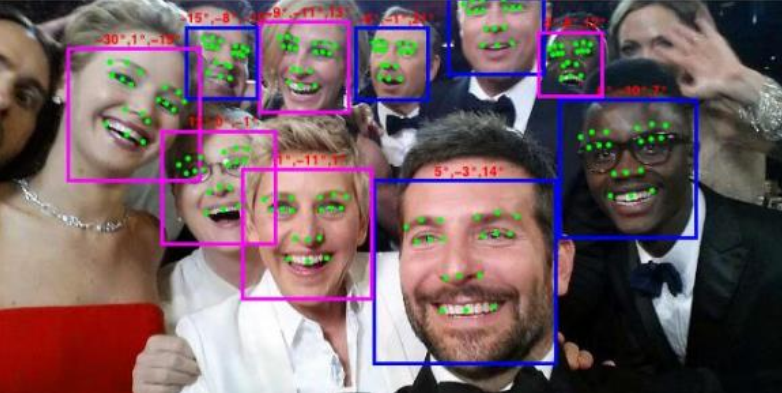
\includegraphics[width=.8\textwidth]{face-detection}
\end{figure}
\end{frame}

\begin{frame}{Face recognition}
Differentiates people, which can be used for identity authentication and privacy protection.
\begin{figure}[!]
\centering
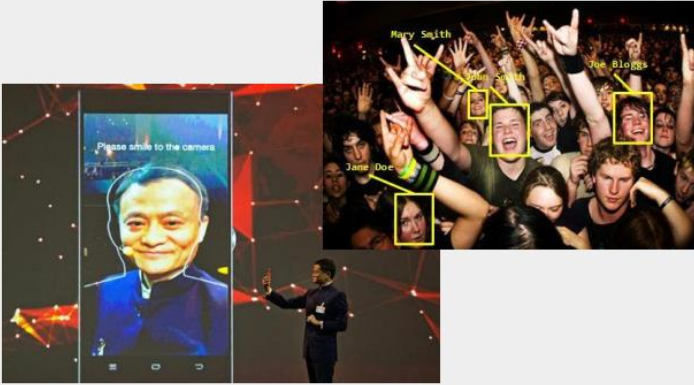
\includegraphics[width=.7\textwidth]{face-recognition}
\end{figure}
\end{frame}

%\begin{frame}{Identification \textit{vs}. Verification}
%Identification \textit{vs}. Verification
%\end{frame}

%\subsection{Object Detection and Recognition}

\begin{frame}{Object Detection and Recognition}
Detects, locates, and identifies different objects in images, including
digital, text, and pedestrian detection. This function can be used for
OCR, unmanned driving, and intelligent image tailoring.
\begin{figure}[!]
\centering
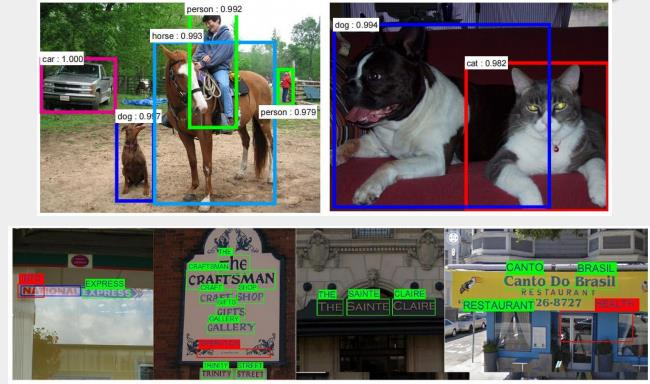
\includegraphics[width=.7\textwidth]{obj-detection-recognition}
\end{figure}
\end{frame}

%\subsection{Semantic Segmentation}

\begin{frame}{Semantic Segmentation}
Predicts the label of each pixel in the image, including segmentation
and recognition. It can be used for unmanned driving, augmented
reality, and situation awareness.
\begin{figure}[!]
\centering
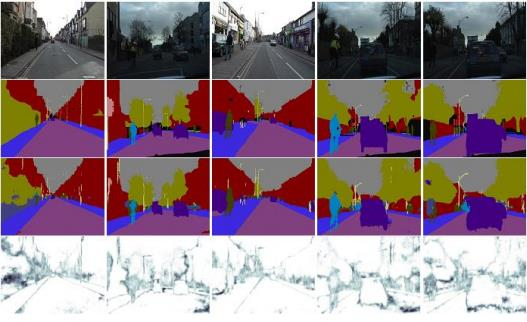
\includegraphics[width=.7\textwidth]{semantic-segmentation}
\end{figure}
\end{frame}

%\subsection{Style Transfer}

\begin{frame}{Style Transfer (Stylization}
Changes the image style while retaining the content of the
image, which can be used for stylized image processing.
\begin{figure}[!]
\centering
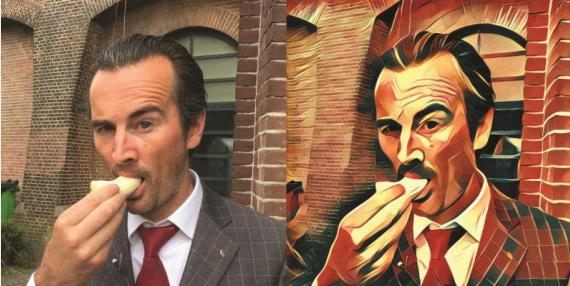
\includegraphics[width=.7\textwidth]{style-transfer}
\end{figure}
\end{frame}

%\subsection{Super-resolution}

\begin{frame}{Super-resolution}
Generates high-resolution images from low-resolution images, which can be
used for image processing, security surveillance, and medical imaging.
\begin{figure}[!]
\centering
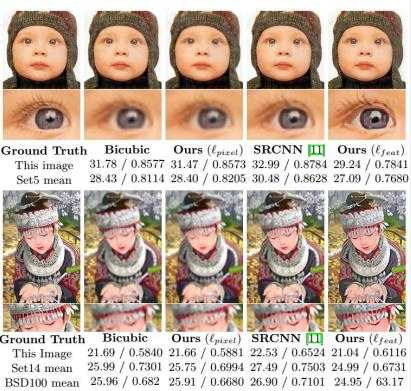
\includegraphics[width=.5\textwidth]{super-resolution}
\end{figure}
\end{frame}

%\subsection{OCR}

\begin{frame}{OCR}
Identifies information such as numbers and texts in images to digitize images or paper documents, which can be used to automatically identify business cards or scan invoices.
\begin{figure}[!]
\centering
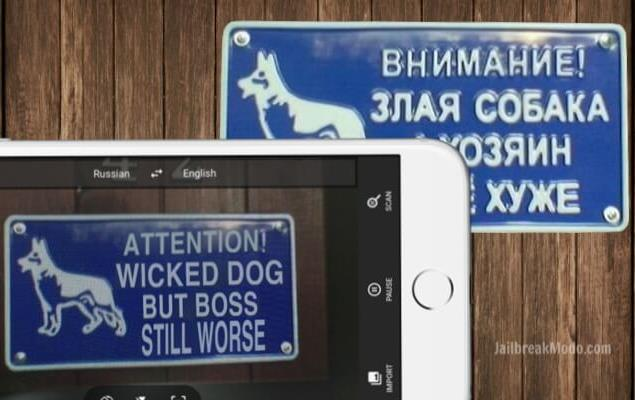
\includegraphics[width=.7\textwidth]{ocr}
\end{figure}
\end{frame}

\section{Natural Language Processing (NLP)}

\begin{frame}{Natural Language Processing (NLP)}
\begin{columns}[t]
\begin{column}{.4\textwidth}
Natural Language Processing
\begin{itemize}
\item Word segmentation.
\item Knowledge exploration.
\item Machine translation.
\item Sentiment analysis.
\end{itemize}
\end{column}
\begin{column}{.6\textwidth}
\begin{figure}[!]
\centering
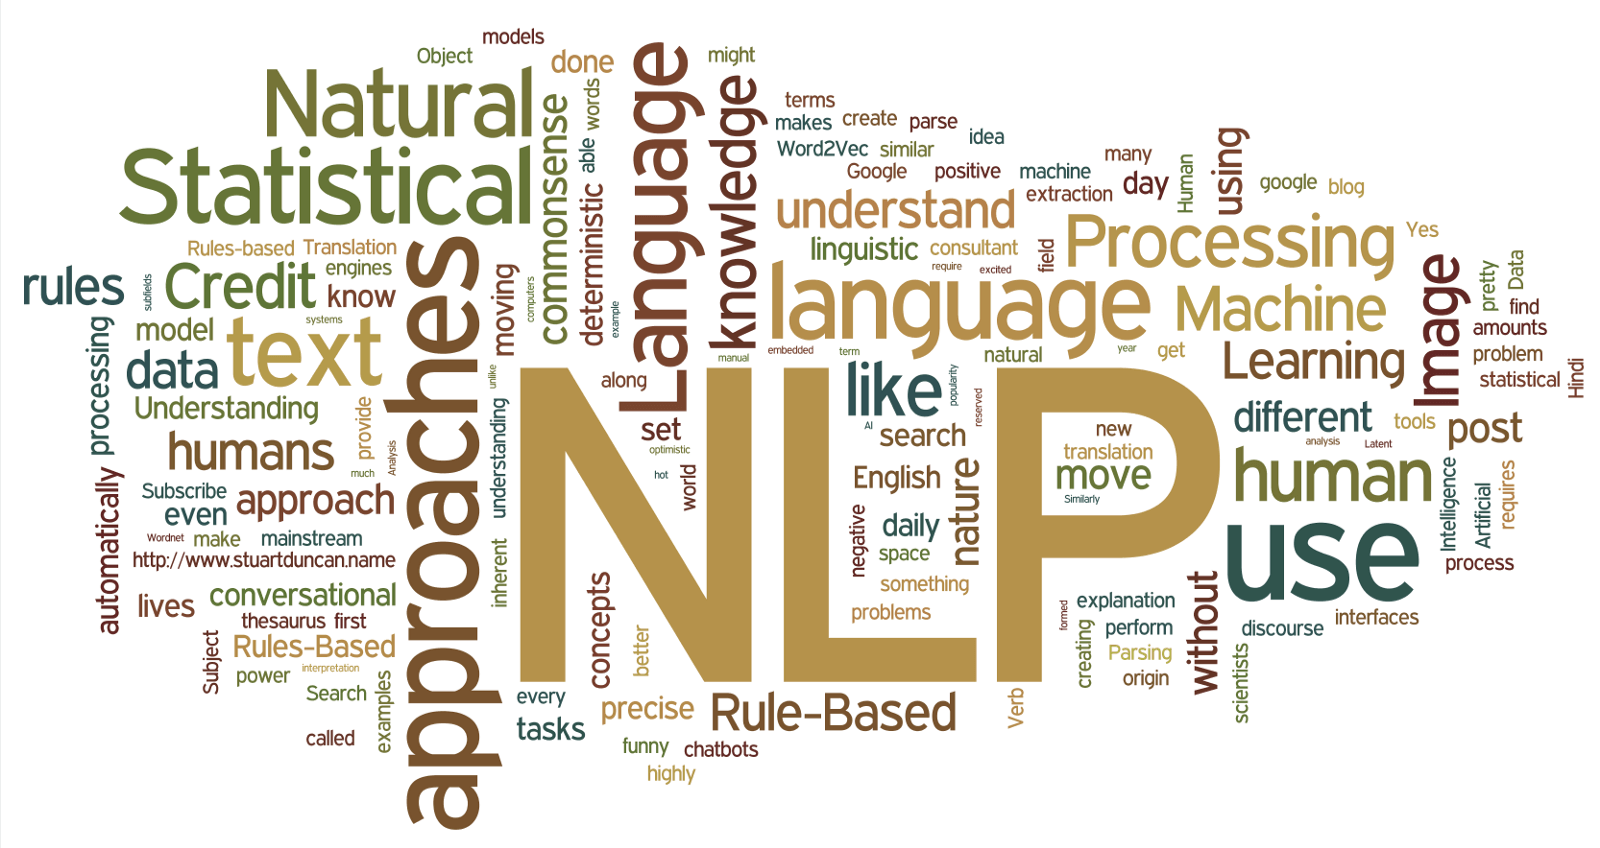
\includegraphics[width=\textwidth]{nlp}
\end{figure}
\end{column}
\end{columns}
\end{frame}

%\begin{frame}{Chinese word-segmenation algorithms}
%\begin{figure}[!]
%\centering
%\includegraphics[width=.7\textwidth]{chinese-word-segmentation-algorithms}
%\end{figure}
%\end{frame}

\begin{frame}{Knowledge Exploration}
\begin{columns}[t]
\begin{column}{.5\textwidth}
Two types of problems:
\begin{itemize}
\item New knowledge reasoning in the existing knowledge base
\begin{itemize}
\item CYC, WordNet, FreeNet, etc.
\item Current studies use similar approaches.
\begin{itemize}
\item Known entities are represented by word embeddings.
\item The entity relationship is modeled using tensor networks.
\item Backpropagation + SGD training.
\end{itemize}
\end{itemize}
\item Mining structured knowledge from free text
\begin{itemize}
\item Text mining
\item TF-IDF
\end{itemize}
\end{itemize}
\end{column}
\begin{column}{.5\textwidth}
\begin{figure}[!]
\centering
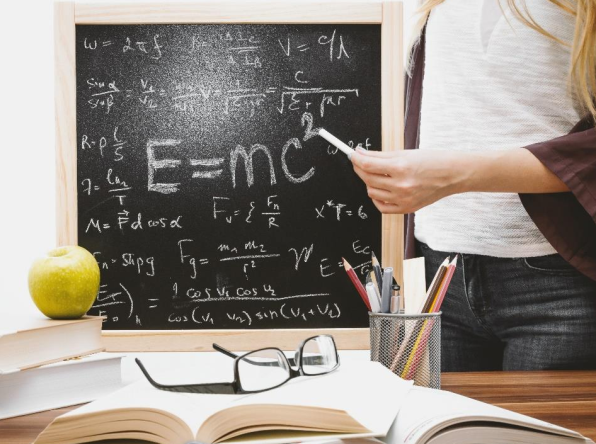
\includegraphics[width=\textwidth]{knowledge}
\end{figure}
\end{column}
\end{columns}
\end{frame}

\begin{frame}{New Knowledge Reasoning in the Existing Knowledge Base}
\begin{figure}[!]
\centering
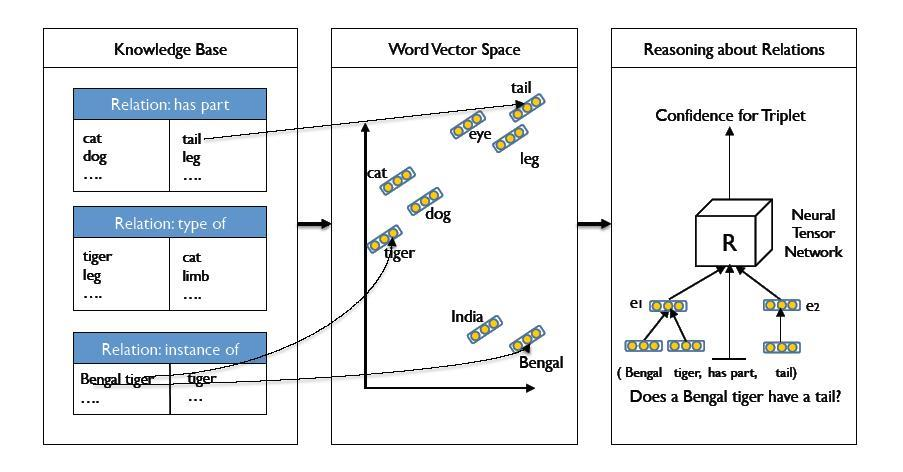
\includegraphics[width=.9\textwidth]{knowledge-base}
\end{figure}
\end{frame}

\begin{frame}{Mining Structured Knowledge from Free Text (1)}
\begin{columns}[t]
\begin{column}{.5\textwidth}
\begin{figure}[!]
\centering
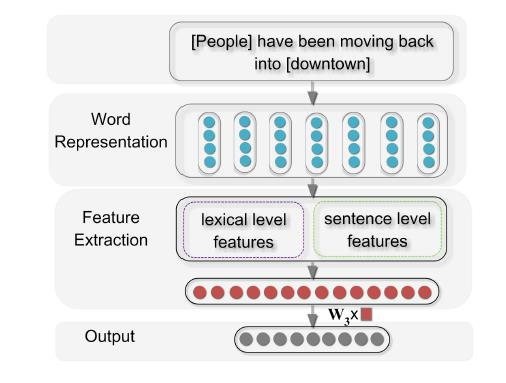
\includegraphics[width=\textwidth]{overall-structure}
\caption{Overall structure}
\end{figure}
\end{column}
\begin{column}{.5\textwidth}
\begin{figure}[!]
\centering
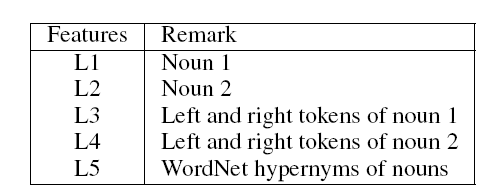
\includegraphics[width=\textwidth]{lexical-feature}
\caption{Lexical feature}
\end{figure}
\end{column}
\end{columns}
\end{frame}


\begin{frame}{Mining Structured Knowledge from Free Text (2)}
Sentence-level feature extraction: convolutional network.
\begin{figure}[!]
\centering
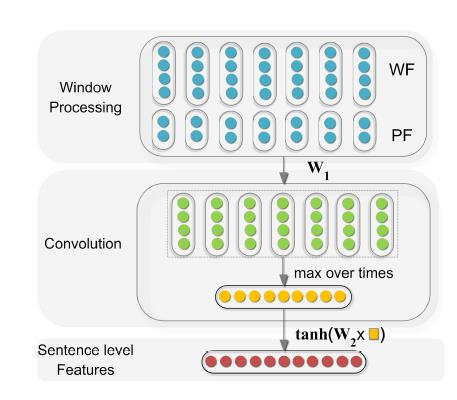
\includegraphics[width=.5\textwidth]{sentence-level}
\end{figure}
\end{frame}

\begin{frame}{Machine Translation (Common Model)}
\begin{itemize}
\item Decoder.
\item Semantic vector.
\item Encoder.
\end{itemize}
\begin{figure}[!]
\centering
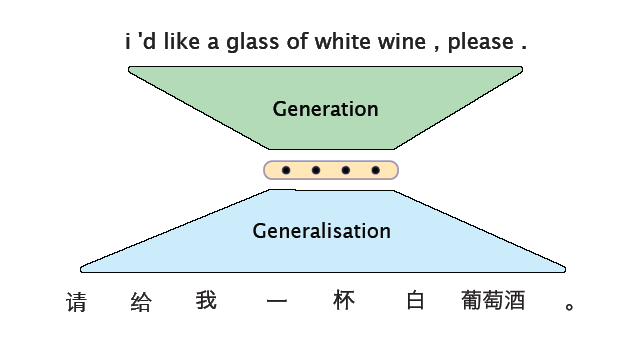
\includegraphics[width=.6\textwidth]{machine-translation}
\end{figure}
\end{frame}

\begin{frame}{Machine Translation: Deep Learning Applied to Multiple Areas}
\begin{columns}[t]
\begin{column}{.4\textwidth}
\begin{itemize}
\item Word alignment
\item Phrase alignment
\item Phrase reordering
\item Language model
\item Translation model
\item Conjunctive model
\item Translation result reordering
\end{itemize}
\end{column}
\begin{column}{.6\textwidth}
\begin{figure}[!]
\centering
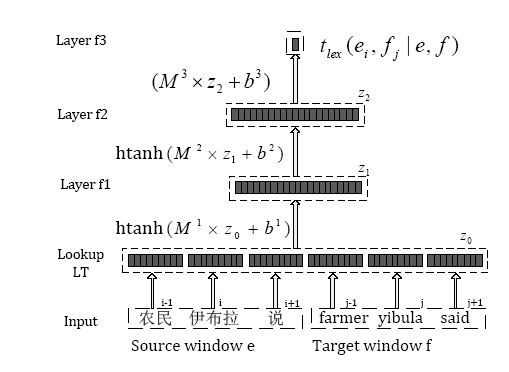
\includegraphics[width=\textwidth]{machine-translation-2}
\end{figure}
\end{column}
\end{columns}
\end{frame}

\begin{frame}{Sentiment Analysis}
Two core issues:
\begin{enumerate}
\item Sentence-level word embedding representation
\item How to encode emotional tendencies to word embedding at all levels
\begin{itemize}
\item Semi-supervised or supervised learning: The emotion tendency is encoded into the WE structure through the training process.
\end{itemize}
\end{enumerate}
\begin{columns}[t]
\begin{column}{.5\textwidth}
\begin{figure}[!]
\centering
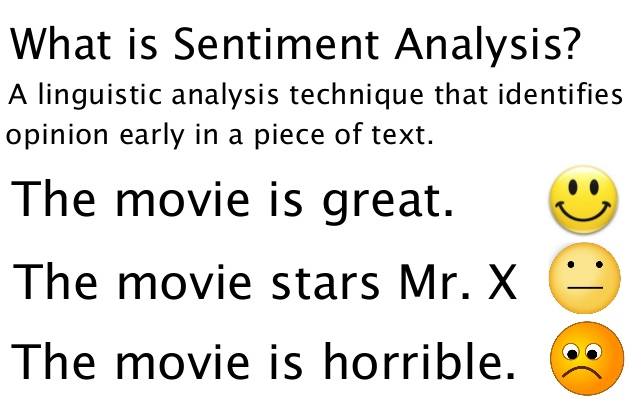
\includegraphics[width=\textwidth]{what-is-sent-analysis-1}
\end{figure}
\end{column}
\begin{column}{.5\textwidth}
\begin{figure}[!]
\centering
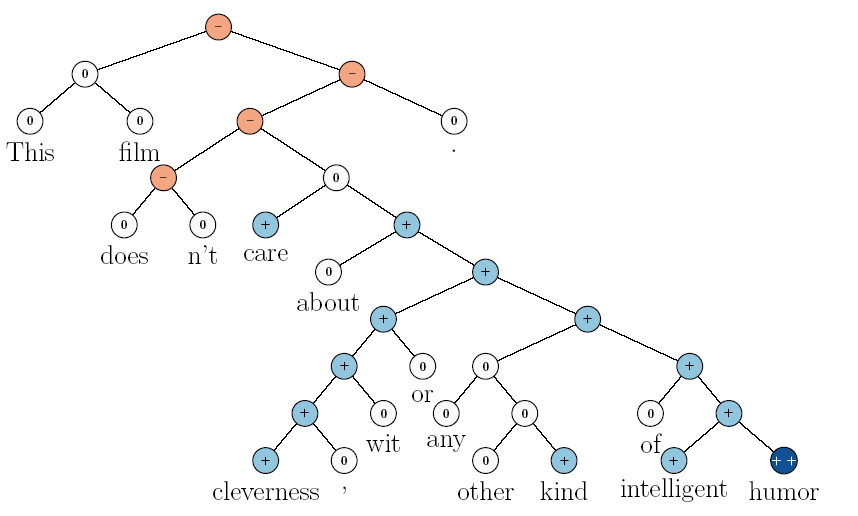
\includegraphics[width=\textwidth]{what-is-sent-analysis-2}
\end{figure}
\end{column}
\end{columns}
\end{frame}

\begin{frame}{Speech Recognition}
\begin{figure}[!]
\centering
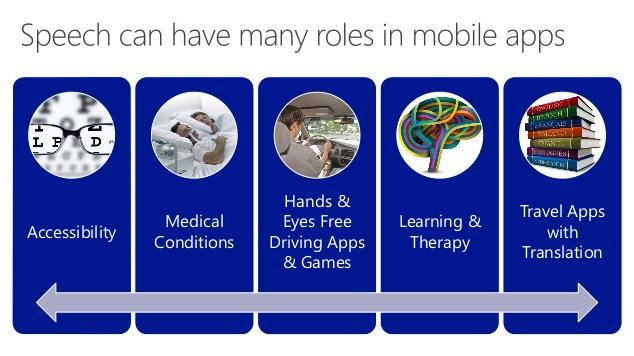
\includegraphics[width=\textwidth]{speech-recognition}
\end{figure}
\end{frame}

\begin{frame}{Recommendation System}
\begin{columns}[t]
\begin{column}{.5\textwidth}
\begin{figure}[!]
\centering
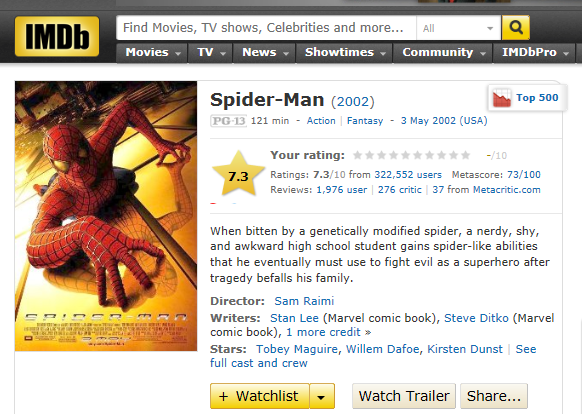
\includegraphics[width=\textwidth]{recommendation-system-1}
\end{figure}
\end{column}
\begin{column}{.5\textwidth}
\begin{figure}[!]
\centering
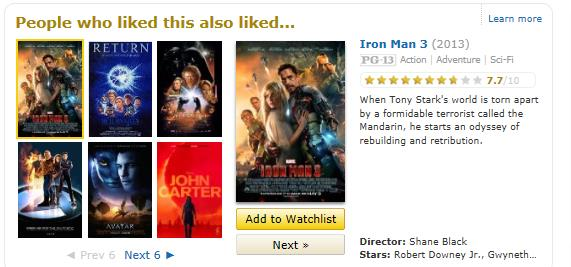
\includegraphics[width=\textwidth]{recommendation-system-2}
\end{figure}
\end{column}
\end{columns}
\end{frame}

\section{Generative Adversarial Networks}


\begin{frame}{}
\begin{figure}[!]
\centering
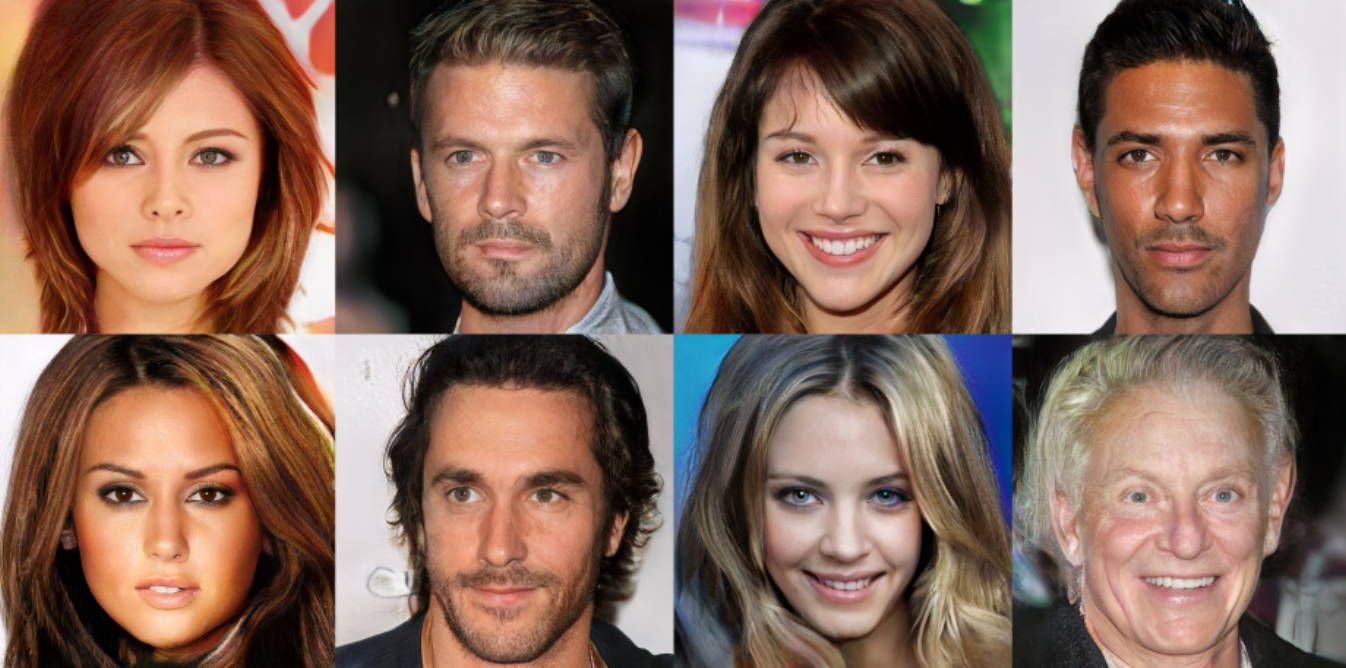
\includegraphics[width=\textwidth]{gan-1}
\end{figure}
\end{frame}


\begin{frame}{}
\begin{columns}[t]
\begin{column}{.5\textwidth}
\begin{figure}[!]
\centering
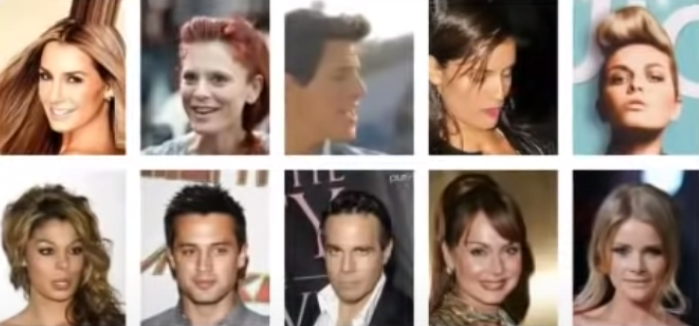
\includegraphics[width=\textwidth]{gan-2}
\end{figure}
\end{column}
\begin{column}{.5\textwidth}
\begin{figure}[!]
\centering
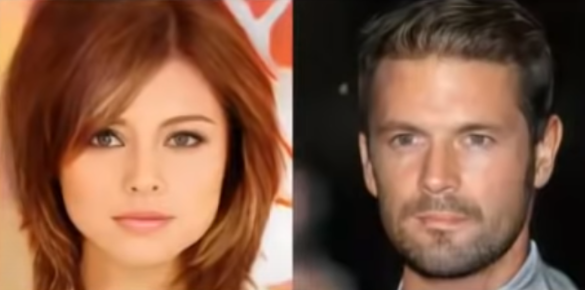
\includegraphics[width=\textwidth]{gan-3}
\end{figure}
\end{column}
\end{columns}
\end{frame}

\begin{frame}{}
\begin{columns}[t]
\begin{column}{.33\textwidth}
\begin{figure}[!]
\centering
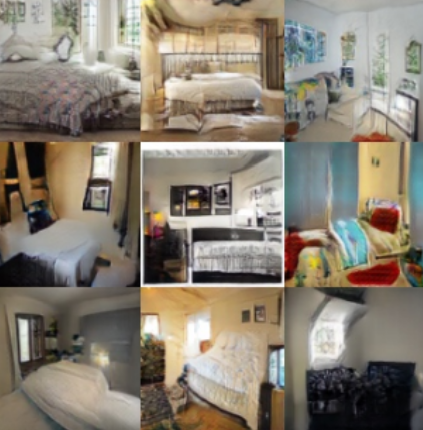
\includegraphics[width=\textwidth]{gan-4}
\end{figure}
\end{column}
\begin{column}{.33\textwidth}
\begin{figure}[!]
\centering
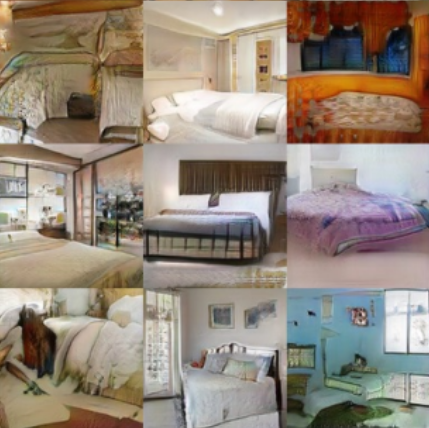
\includegraphics[width=\textwidth]{gan-5}
\end{figure}
\end{column}
\begin{column}{.33\textwidth}
\begin{figure}[!]
\centering
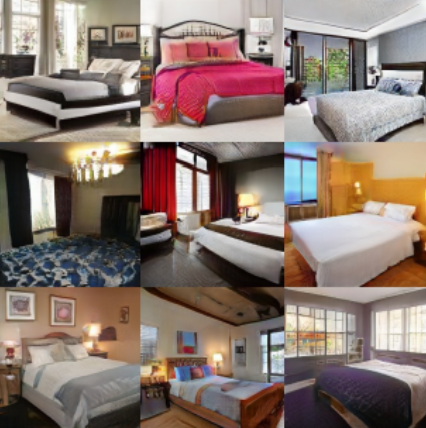
\includegraphics[width=\textwidth]{gan-6}
\end{figure}
\end{column}
\end{columns}
\end{frame}


\begin{frame}{}
\begin{figure}[!]
\centering
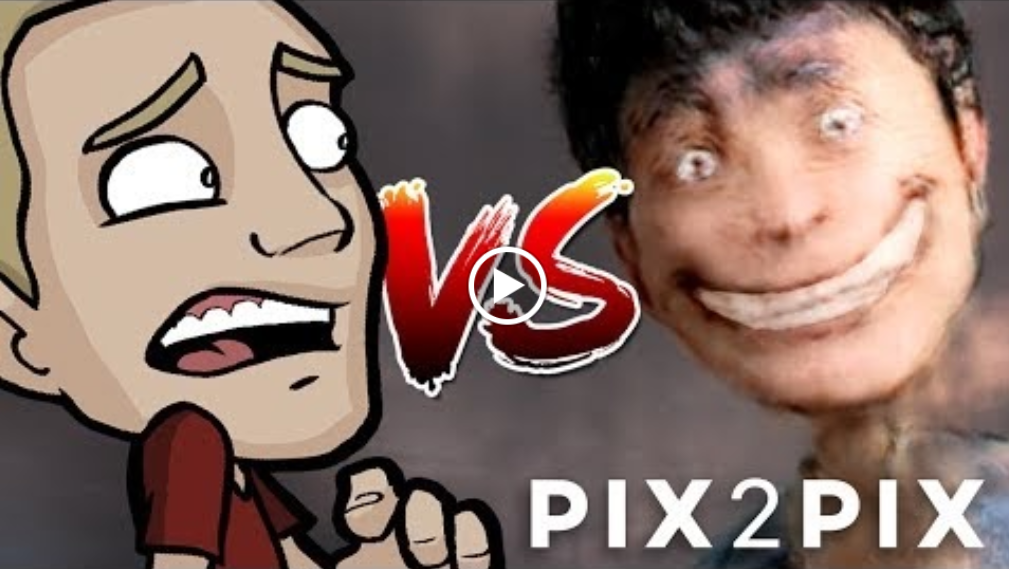
\includegraphics[width=\textwidth]{pix2pix}
\end{figure}
	\end{frame}


\begin{frame}{}
\begin{figure}[!]
\centering
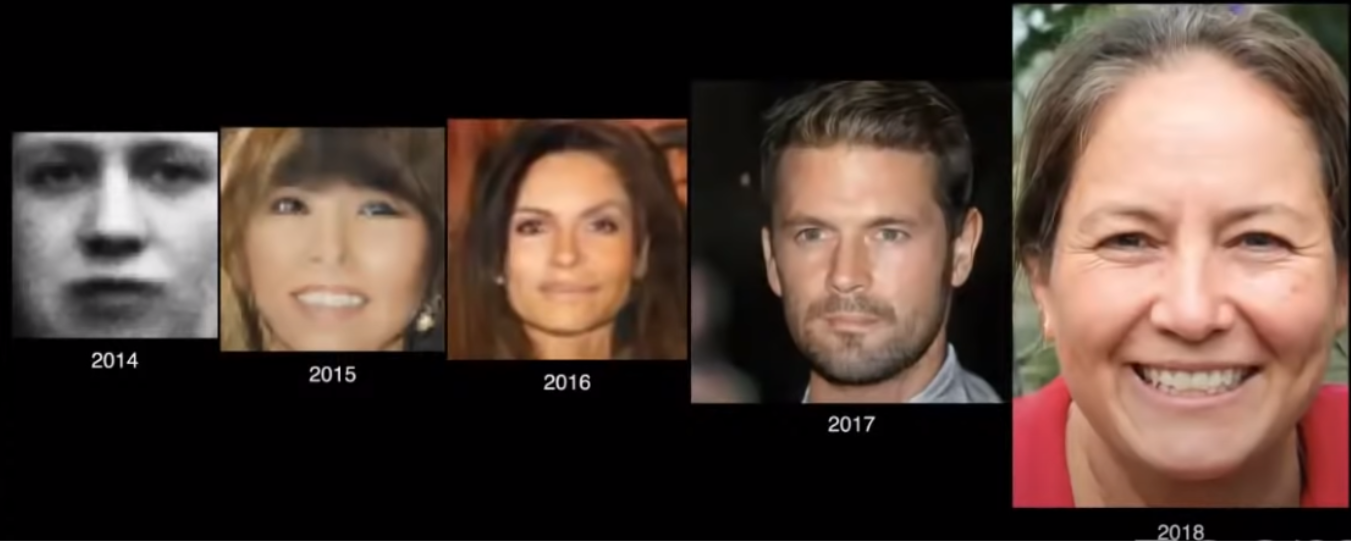
\includegraphics[width=\textwidth]{gan-evolution}
\end{figure}
\end{frame}


\begin{frame}{}
\begin{figure}[!]
\centering
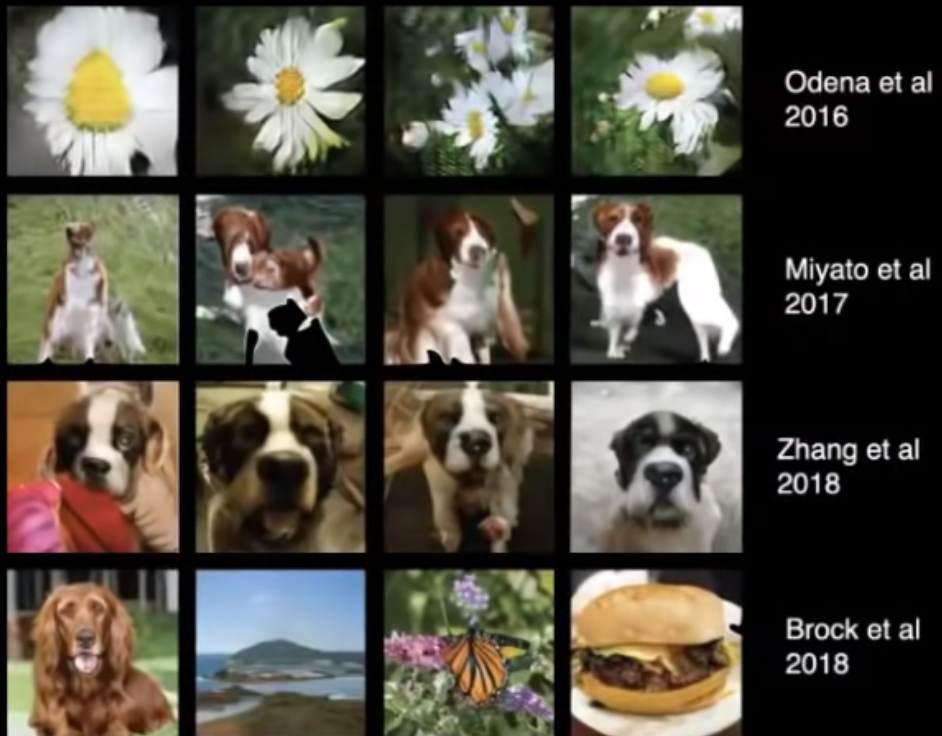
\includegraphics[width=\textwidth]{gan-evolution-2}
\end{figure}
\end{frame}

\begin{frame}{}
\begin{figure}[!]
\centering
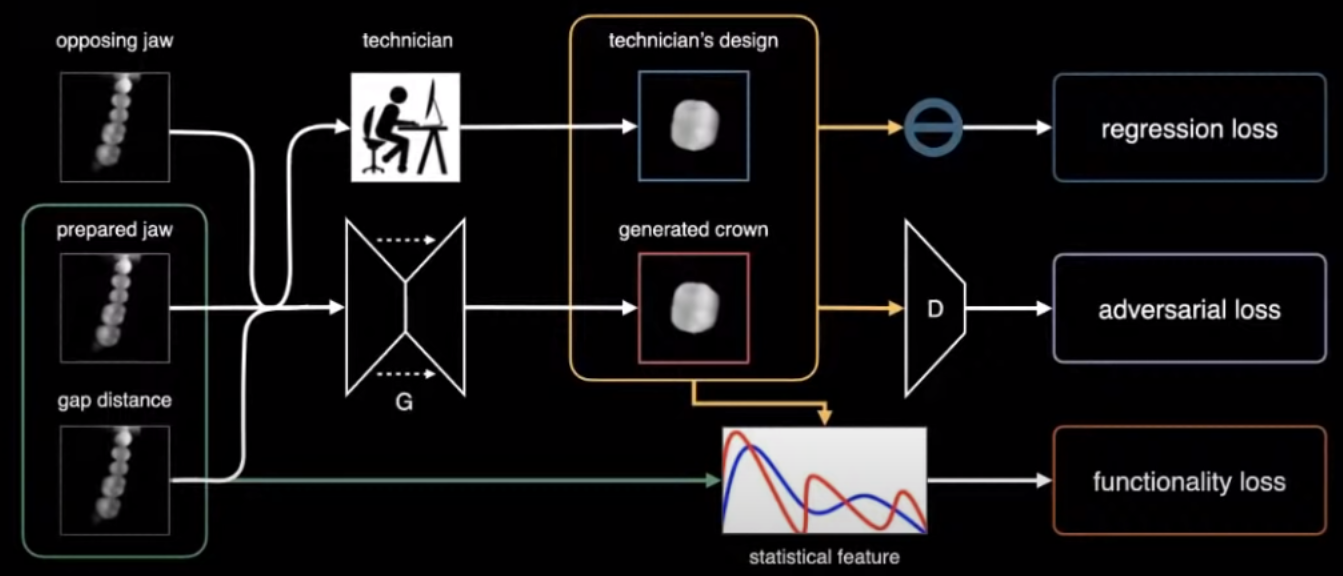
\includegraphics[width=\textwidth]{gan-crown}
\end{figure}
\end{frame}


%\begin{frame}{}
%\begin{figure}[!]
%\centering
%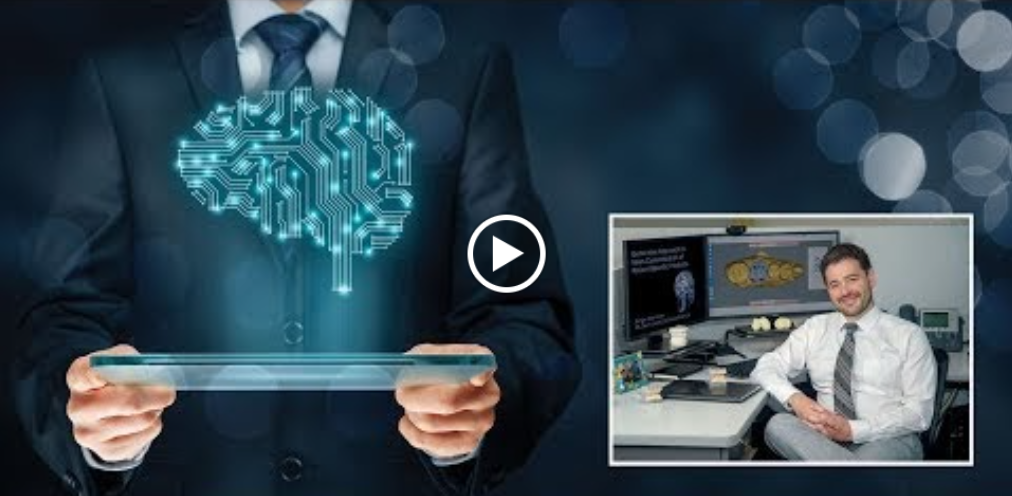
\includegraphics[width=\textwidth]{gan-video}
%\end{figure}
%\end{frame}


\begin{frame}{}
\begin{figure}[!]
\centering
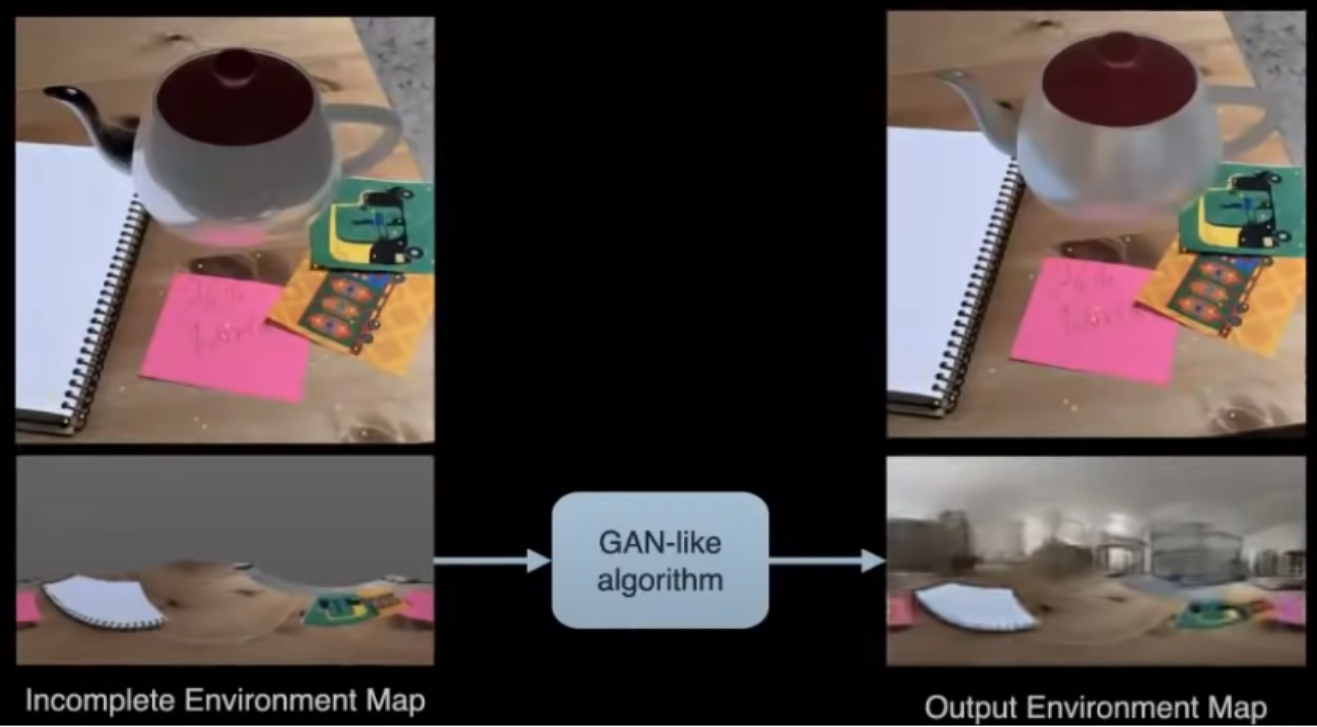
\includegraphics[width=\textwidth]{gan-ar}
\end{figure}
\end{frame}


\begin{frame}
\frametitle[alignment=center]{}
\flushbottom
\centering
Thank you!\\
\href{mailto:tiago@ic.ufal.br}{tvieira@ic.ufal.br}\\
%\href{mailto:warley.barbosa@edge.ufal.br}{warley.barbosa@edge.ufal.br}\\
%\href{mailto:icaro.bastos@edge.ufal.br}{icaro.bastos@edge.ufal.br}\\
\end{frame}


\end{document}
